%SOP Template 
% Version 02 Added revision date
% Version 03 Added TOC and acknowledgements
%           New SOP4_alpha.cls
% Version 04 Revised Order and Simplifed SOP


\documentclass[12pt]{../SOP4_alpha}\usepackage[]{graphicx}\usepackage[]{color}
%% maxwidth is the original width if it is less than linewidth
%% otherwise use linewidth (to make sure the graphics do not exceed the margin)
\makeatletter
\def\maxwidth{ %
  \ifdim\Gin@nat@width>\linewidth
    \linewidth
  \else
    \Gin@nat@width
  \fi
}
\makeatother

\definecolor{fgcolor}{rgb}{0.345, 0.345, 0.345}
\newcommand{\hlnum}[1]{\textcolor[rgb]{0.686,0.059,0.569}{#1}}%
\newcommand{\hlstr}[1]{\textcolor[rgb]{0.192,0.494,0.8}{#1}}%
\newcommand{\hlcom}[1]{\textcolor[rgb]{0.678,0.584,0.686}{\textit{#1}}}%
\newcommand{\hlopt}[1]{\textcolor[rgb]{0,0,0}{#1}}%
\newcommand{\hlstd}[1]{\textcolor[rgb]{0.345,0.345,0.345}{#1}}%
\newcommand{\hlkwa}[1]{\textcolor[rgb]{0.161,0.373,0.58}{\textbf{#1}}}%
\newcommand{\hlkwb}[1]{\textcolor[rgb]{0.69,0.353,0.396}{#1}}%
\newcommand{\hlkwc}[1]{\textcolor[rgb]{0.333,0.667,0.333}{#1}}%
\newcommand{\hlkwd}[1]{\textcolor[rgb]{0.737,0.353,0.396}{\textbf{#1}}}%
\let\hlipl\hlkwb

\usepackage{framed}
\makeatletter
\newenvironment{kframe}{%
 \def\at@end@of@kframe{}%
 \ifinner\ifhmode%
  \def\at@end@of@kframe{\end{minipage}}%
  \begin{minipage}{\columnwidth}%
 \fi\fi%
 \def\FrameCommand##1{\hskip\@totalleftmargin \hskip-\fboxsep
 \colorbox{shadecolor}{##1}\hskip-\fboxsep
     % There is no \\@totalrightmargin, so:
     \hskip-\linewidth \hskip-\@totalleftmargin \hskip\columnwidth}%
 \MakeFramed {\advance\hsize-\width
   \@totalleftmargin\z@ \linewidth\hsize
   \@setminipage}}%
 {\par\unskip\endMakeFramed%
 \at@end@of@kframe}
\makeatother

\definecolor{shadecolor}{rgb}{.97, .97, .97}
\definecolor{messagecolor}{rgb}{0, 0, 0}
\definecolor{warningcolor}{rgb}{1, 0, 1}
\definecolor{errorcolor}{rgb}{1, 0, 0}
\newenvironment{knitrout}{}{} % an empty environment to be redefined in TeX

\usepackage{alltt}

\usepackage[english]{babel}


\title{Trilogy Laboratory Fluorometer}
\date{06/10/2019}
\author{Marc Los Huertos}
\approved{TBD}
\ReviseDate{\today}
\SOPno{18v4}
\IfFileExists{upquote.sty}{\usepackage{upquote}}{}
\begin{document}


\maketitle

\section{Scope and Application}

\NP The purpose of this SOP is to train researchers in the use of the Trilogy Laboratory Fluorometer, a compact, multifunctional laboratory instrument that can be used for making fluoresence, absorbance, or turbidity measurements using the appropriate snap-in Optical Module. 

\section{Summary of Method}

\NP The Trilogy Laboratory Fluorometer is a compact, multifunctional laboratory insturment that can be used for making fluoresence, absorbance, and turbidity measurements using the appropriate snap-in Optical Module. A color touch screen with simple menus makes for an intuitive user interface. 

\NP When properly calibrated, the Trilogy Fluorometer will read out the concentration of the solution. 

\NP Optical Modules contain the necessary light source and filters for the relevant application. 

\tableofcontents

\newpage

\section{Scope and Application}

\section{Summary of Instrument Use}


\section{Acknowledgements}

This SOP was orginally written by Isaac Medina and then substantially updated and improved by Virginia Paschal. 

\section{Defintions}

\section{Biases and Interferences}



\section{Health and Safety}

\NP Describe the risk...


\subsection{Safety and Personnnel Protective Equipment}

\section{Personnel \& Training Responsibilities}

\NP Researchers training is required before this the procedures in this method can be used... 

\NP Researchers using this SOP should be trained for the following SOPs:

\begin{itemize}
  \item SOP01 Laboratory Safety
\end{itemize}

\section{Required Materials and Apparti}

\NP The Trilogy accommodates 10 x 10 mm methacrylate and polystyrene cuvettes (minimum 2mL volume). 

\NP Use 12 mm x 35mm glass test tubes for extracted chlorophyll measurements, and use methacrylate for ammonium measurements.

\NP The Absorbance Module accommodates 10 x 10 mm methacrylate and polystyrene cuvettes as well as glass cuvettes (minimum 1.5 mL volume).

\NP Use Polystyrene curvettes for measuring turbidity.

\section{Reagents and Standards}

\section{Estimated Time}

\section{Sample Collection, Preservation, and Storage}

\section{Procedures}

\subsection{Preparing to Analyze Samples}

\NP Turn on Instrument.

\begin{figure}
  \centering
  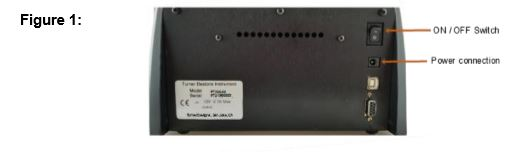
\includegraphics[width=0.7\textwidth]{Capture}
  \caption{The instrument is turned on at the back.}
  \label{fig:capture}
\end{figure}

\subsection{Determine and Select Appropriate Modules and Modes}

The following modules are available for the Fluorometer: Absorbance Module, Turbidity Module, and Fluorecence Module. 

\NP Install the appropriate module as shown in Figure~\ref{fig:module}. 

\begin{figure}
  \centering
  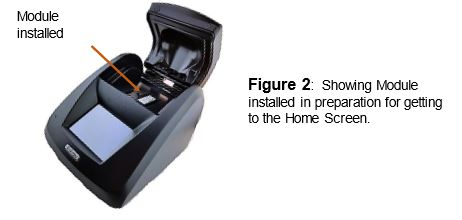
\includegraphics[width=0.7\textwidth]{Capture2}
  \caption{Fluorometer with a module installed.}
  \label{fig:module}
\end{figure}

\NP After installing the module, use the menu to define mode???

\begin{description}
  \item[Absorbance Module] accepts interchangeable filter paddles so measurements can be made at different wavelenghts in order to identify or place a sample in a particular class of compounds. 
  The standard filter paddle (Figure~\ref{fig:filterpaddle}) wavelengths/bandwidths are: 560/10; 600/10 and 750/10 nm.
  
\begin{figure}
  \centering
  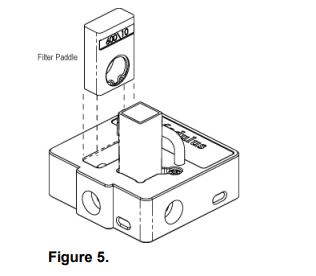
\includegraphics[width=0.7\textwidth]{figure5}
  \caption{Filter paddle installation.}
  \label{fig:filterpaddle}
\end{figure}

  \NP There are two measurment modes available on the Trilogy when using the Absorbance Module:
\begin{itemize}
  \item 1. Raw Mode: No calibration required
  \item 2. Direct Concentration Mode: Calibration required
\end{itemize}
  
  
  \item[Turbidity Module] uses an Infrared (IR) LED with a wavelength of 850 nm as required for reference method: ISO 7027/DIN EN 27027, "Water Quality- Determination of Turbidity" (Figure~\ref{fig:trubiditymenu}). Using Infrared allows Turbidity to be measured at wavelengths that are not normally absorbed by organic matter thereby reducing susceptibility to interference by sample color. 

\begin{figure}
  \centering
  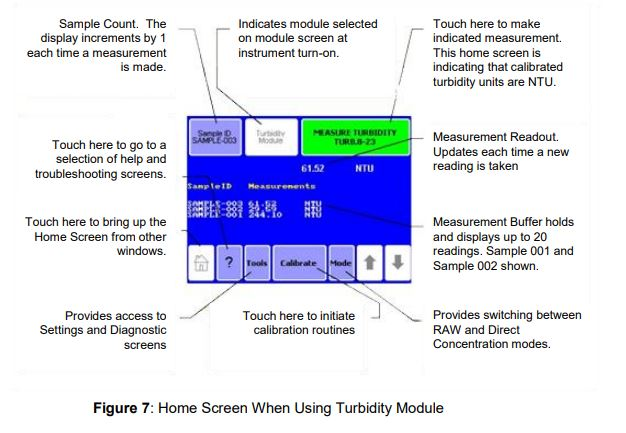
\includegraphics[width=0.7\textwidth]{figure6turbidity}
  \caption{Fluorometer menu with turbidity module installed.}
  \label{fig:trubiditymenu}
\end{figure}  
  
  
  \NP Two measurement modes are avaliable on the Trilogy when using the Turbidity Module:

\begin{description}
\item[Raw Mode] should be used for qualitative measurement, for example where measuring changes is required, rather than absolute concentration values. Readings are displayed in Nephelometric Turbidity Units (NTU).
  \item[Direct Concentration Mode] The Direct Concentration mode makes absolute measurements based on a calibration.
\end{description}

  \item[Fluoresence Module]
  
(Figure~\ref{fig:modulemenu}).

\begin{figure}
  \centering
  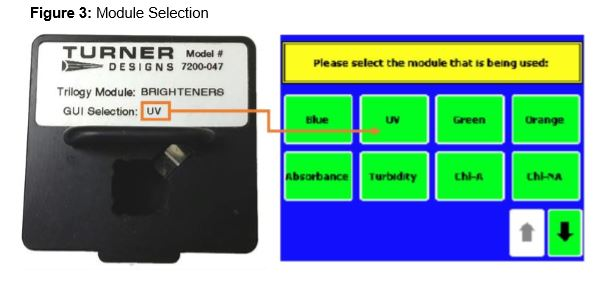
\includegraphics[width=0.7\textwidth]{Capture3}
  \caption{Fluorometer menu with a florescence module installed.}
  \label{fig:modulemenu}
\end{figure}

\NP Two measurement modes are avaliable on the Trilogy when using the Fluoresence Module:

\begin{itemize}
  \item Raw Fluoresence Mode: No calibration required. The Raw Fluoresence Mode should be used for qualitative measurement, for example where measuring changes is required, rather than absolute concentration values. Readings are displayed in Relative Fluoresence Units (RFU).
  \item Direct Concentration Mode: Direct Concentration Mode: The Direct Concentration mode makes absolute measurements based on a calibration (see Calibration Overview).
\end{itemize}

\NP Touch "Mode" on the Home Screen to select the measurement mode (Figure~\ref{fig:fluoresencemode}).

\begin{figure}
  \centering
  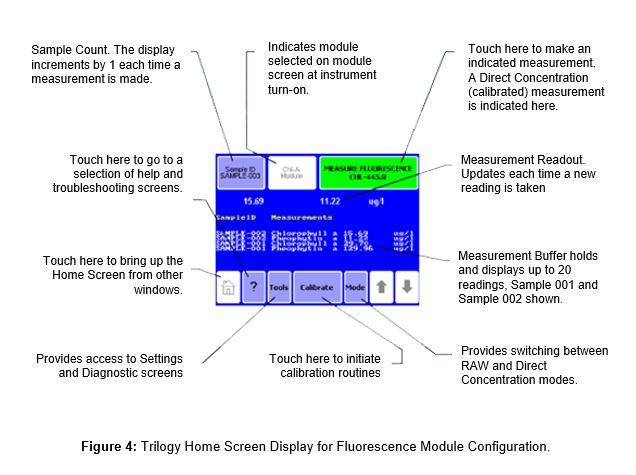
\includegraphics[width=0.7\textwidth]{Capture4}
  \caption{Fluoresence Mode Selection Module.}
  \label{fig:fluoresencemode}
\end{figure}

\NP EPA Method 445.0 is a standard method for measuring extracted chlorophyll a and pheophythin a in marine and fresh water algae by fluroescence. It requires extraction with 90 percent acetone, measurements before and after acidification and some fairly simple calculations to arrive at the chlorophyll a and pheophytin concentrations.

\NP A known concentration of pure chlorophyll $\alpha$ (as a standard) is required at least the first time you calibrate Trilogy. For greatest accuracy however, we recommend that you periodically (once every few months) use a known concentration of pure chlorophyll $\alpha$ in 90 percent acetone to recalibrate your instrument. 


\end{description}



\subsection{Mode Selection -- Absorbance}



\subsection{Mode Selection -- Turbidity}



\subsection{Mode Selection -- Fluoresence}



\subsection{Single Sample Measurements}

\NP Open the lid of the trilogy and insert the cuvette. Close the lid.

\NP Touch "Sample ID" to name your sample (optional).

\NP Using the keypad, enter the sample name into the name field. Touch "Save" to save the sample ID.

\NP Touch "Measure Fluoresence" / "Measure Absorbance" / "Measure Turbidity" depending on the installed module.

\NP The Trilogy will measure the sample for 6 seconds and report the average reading for the sample. 

\NP The Trilogy reports data on the "Home" screen and displays the results for the most recent 20 measurements. 

\NP Use the arrow keys to scroll through the most recent measurements. The data automatically exports to a printer or PC when properly connected. 

\NP Please note the Trilogy does NOT store more than 20 measurements at one time. If more than 20 readings are taken, the oldest reading will be overwritten. 

\NP Measurements are not stored between power cycles. 

\subsection{Continuous Measurments}

\NP The Continuous Sampling feature enables repeat measurements at user-defined intervals.

\NP Touch "Continuous Sampling" and turn the feature ON. Highlight the frequency of measurement and the numnber of total measurements. The maximum number of total measurements is 9999.

\NP Touch "OK" to return to the "Home" screen.

\NP Connect the Trilogy to a printer or a PC to collect the data. Touching the screen repeatedly causes an early-abort of Continuous Sampling measurments. 


\section{Data Analysis and Calculations}

\NP When properly calibrated, the Trilogy Fluorometer will read out the actual concentration of the solution.

\section{QA/QC Criteria}

\subsection{Calibration Overview}

\NP The Trilogy calibration procedure calculates the fluorescent signal to your units of measure. Once calibrated, the Trilogy can give you concentration readings directly, saving you from having to perform any calculations. 

\subsection{When to Calibrate?}

\begin{enumerate}
  \item For greatest accuracy, calibrate before running a new batch of samples.
  \item Recalibrate if the ambient temperature changes by +/- 5 degrees Celsisus.
  \item Recalibrate after changing to a different optical module, or if you make measurements on a new analyte. 
  \item Verify the need to calibrate by reading a stable, known concentration standard immediately after calibration and again every few hours to see if readings have changed significantly. Recalibrate when the accuracy beomes unacceptable for your study.
\end{enumerate}

\subsection{Trilogy Calibration Options and Procedures}

\NP There are two measurement modes available on the Trilogy when using either the Fluoresence or Turbidity Modules:

\begin{enumerate}
  \item Raw Fluoresence Mode - No calibration required
  \item Direct Concentration Mode - Calibration required 
\end{enumerate}

\subsection{Raw Fluorescence Mode}

\NP The Raw Fluorescence Mode should be used for qualitative measurement, for exmaple where measuring changes is required, rather than absolute concentration values. Readings are displayed in Relative Fluorescence Units RFU.

\NP A calibration is not necessary to measure fluorescence with the Trilogy. Simply use the Raw Fluorescence Mode to obtain the fluorescent value of a sample in Relative Fluorescence Units (RFU). 

\NP Use the standard curve to determine the concentration of the analyte in the samples. The Trilogy does not manipulate the data while operating in the Raw Fluorescence Mode. 

\NP It is not necessary to zero the Trilogy for use in the Raw Fluorescence Mode, however a blank sample should be run to determine background fluorescence. A solid secondary standard may be used to verify instrument stability and function.

\subsection{Direct Concentration Calibration}

\NP Direct Concentrations can be calibrated by using single or multi-point calibrations. In multi-point calibrations, up to five standards and a blank can be read generating a calibration curve for superior accuracy. The software uses these points to calculate direct concentrations. The Trilogy will display the actual concentration of your samples in units that were choosen during calibration. 

\NP The Direct Concentration Mode requires a calibration with one blank solution and at least one standard solution. 

\NP The following procedure applies to all the fluorescence modules with the exception of the Chl Acidification and Non-Acidification modules. (There are separate procedures for these two exceptions). 

\NP The procedure requires the use of at least one calibration standard, (Chlorophyll a, Rhodamine WT, etc.). Up to 5 standard solutions can be used for a Multi Point Calibration. Calibrations can be given a name and stored for future use. 

\subsection{"Direct Calibration" Procedure}

\NP "Direct Calibraiton" can be used for the fluoresence and turbidity modules, single point and multi point calibrations.

\NP The following procedure applies to Trilogy and the Fluoresence or Turbidity Modules.

\NP Turn on the Trilogy

\NP Select the module/application to be calibrated and confirm by touching "OK".

\NP On the home screen, touch "Calibrate" to begin a calibration sequence.

\NP Select "Run New Calibration"

\NP Select the unit of measurement 

\NP Insert the calibration "blank" and touch "OK"

\NP Enter the concentration for the first Standard. If using the Turner Designs Chlorophyll a Standard, this will be the concentration data supplied with the Standard. If doing multi point calibrations, be sure to use Standards in order of increasing concentration.

\NP Follow the screen prompt indicating that the standard should be inserted, touch OK.

\NP After the calibration is complete, either select "Proceed with Current Calibration" or select "Enter More Standards", in whcih case, return to the previous step.

\NP Save the calibration for future use (optional).

\NP Subsequent readings in the Direct Concentration mode reflect the actual concentration of the analyte. 

\NP Confirm successful completion of the calibration by measuring the same Standard. The displayed concentration should equal the value used in step 7. Optionally, the Solid Secondary Standard could now be adjusted to give the same reading for future calibrations.



\section{Trouble Shooting}
\subsection{Fluorescence Troubleshooting}
\begin{itemize}
  \item SYMPTOM: Bad calibration error message
  \item POSSIBLE SOLUTIONS: A bad calibration error message may occur if the blank is brighter than the standard. Compare the reading of the standard and the blank in the Raw mode. 
  \item SYMPTOM 2: Erratic reading
  \item POSSIBLE SOLUTIONS: When direct fluoresence readings do not produce expected values, review the standard value entered during the calibration. The number of the standard value should correspond to the actual concentration of the standard.
  \item SYMPTOM 3: Negative values
  \item POSSIBLE SOLUTIONS: After calibration, the blank value is automatically subtracted from subsequent readings. A negative reading can occur if a sample reading is less than the bank.
  \item SYMPTOM 4: Low readings
  \item POSSIBLE SOLUTIONS: Check the excitation and emission wavelengths of the analyte against the specifciations of the Fluorescence Optical Application Module in use. Different analytes require different Optical Application Modules.
  \item SYMPTOM 5: High Background
  \item POSSIBLE SOLUTIONS: A wet cuvette or spill could contaminate the cuvette holder and increase the background signal. Carefully clean the cuvette holder with 70 percent ethanol. 
\end{itemize}

\subsection{Absorbance Troubleshooting}
\begin{itemize}
  \item SYMPTOMS: Non-Linear Response
  \item POSSIBLE SOLUTIONS: Many absorbance assays do not produce a linear response but instead produce a sigmoidal or pseudo-sigmodial response. 
  \item SYMPTOM 2: Low Readings
  \item POSSIBLE SOLUTIONS: Check the filter installed in the Absorbance Module and make sure it is the correct filter for the assay. View the Calibration details from the Tools menu.
  \item SYMPTOM 3: Bad Calibration Error Message
  \item POSSIBLE SOLUTIONS: Install the proper filter and use the ultrapure water in a clean cuvette to update the zero. Check the Calibration detais from the Tools menu. 
\end{itemize}

\subsection{Turbidity Troubleshooting}
\begin{itemize}
  \item SYMPTOMS: Trilogy readings do not agree with other Turbidity meters
  \item POSSIBLE SOLUTIONS: Calibrate both meters with the same calibration standard solution. If meters still display significantly different readings, it may be that the second turbidity meter does not make an IR measurement, and the sample contains interfernce colors. 
  \item SYMPTOMS 2: The turbidity readings change each time a reading is taken
  \item POSSIBLE SOLUTIONS: This is normal. Particles in a liquid sample do not remain in the same position, and these position changes affect the scattering of the light, and therefore the turbidity reading. 
  \item SYMPTOMS 3: My turbidity readings seem to be different when I recalibrated with a new primary standard.
  \item POSSIBLE SOLUTIONS: Formazine standards from the basis of all turbidity measurements and they are very susceptible to aging. ISO 7027 recommendation specifies that the 4,000 NTU Formazine solution can be kept for only 4 weeks. For consistent readings calibrate with current standards. 
\end{itemize}

\section{References}

\NP APHA, AWWA. WEF. (2012) Standard Methods for examination of water and wastewater. 22nd American Public Health Association (Eds.). Washington. 1360 pp. (2014).

\end{document}
